\chapter{An\'{a}lisis y dise\~{n}o}
%\newpage
%Cómo se plantea el desarrollo del trabajo. En que partes se 
%divide la solución, justificando dicha división y explicando 
%cada una de las partes.

%En aquellos trabajos donde sea aplicable se documentará 
%usando el modelo de dominio, el diagrama de clases, los 
%módulos/paquetes del software desarrollado, etc.

\section{An\'{a}lisis}
Los datos que recoge el software est\'an en un XML. El XML describe los datos que han de mostrarse. A grosso modo se dividen en:
\begin{itemize}
	\item Observaciones
	\item Propiedades
	\item Instantes
\end{itemize}

Por tanto se ha decidido guardar la lista de Observaciones, la lista de Propiedades para cada Observaci\'on y cada Propiedad
una lista de Instantes en los que se guardar\'a los valores.

Como cada observaci\'on tiene muchas propiedades, es un requisito que las propiedades est\'en
agrupadas por observaci\'on.

El rango seleccionado en cada propiedad estar\'a sincronizado con el resto de propiedades cargadas. 
Ya que no tiene sentido que por ejemplo, la observaci\'on ``coche", 
que tiene como propiedades ``velocidad" \ y ``aceleraci\'on" \ tengan distintos rangos 
seleccionados, ya que si en ``velocidad" \ seleccionamos [1, 3] y en ``aceleraci\'on" \ [3, 4], 
¿Qu\'e guardamos? ¿El primero o el segundo? Por tanto, ya que todas las propiedades suceden al
mismo tiempo se sabe que est\'an relacionadas, por lo que es necesario que los rangos est\'en
seleccionados.

A la hora de guardar, tampoco podr\'an guardarse distintos rangos que se solapen con los
previamente creados. Ya que en un mismo instante de tiempo, no pueden estar sucediendo dos cosas al mismo tiempo.
Por ejemplo, un brazo no puede estar levant\'andose, y baj\'andose al mismo tiempo.

Gr\'aficamente las clases se dividen de dos maneras: Contenedores y clases ``hoja".
El programa puede verse como una estructura de \'arbol, en las que de la ventana principal,
cuelgan los contenedores de v\'ideo y gr\'aficos, de los de gr\'aficos cuelga el 
visualizador de datos.

\section{Dise\~{n}o}

\subsection{Diagrama de clases}

\subsection{Listado de m\'odulos}

\subsection{Diagrama de casos de uso extendidos}
En el diagrama de casos de uso, se puede ver que acciones puede realizar el usuario en cualquier momento, y cuales
est\'an supeditadas a ciertas condiciones. N\'otese que las condiciones de los ``extend" \ son los comentarios a\~nadidos
a los subcasos de uso.

\begin{figure}[h]
\centering
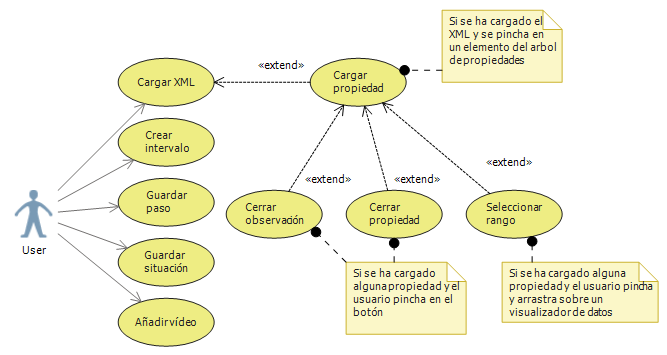
\includegraphics[width=1.0\linewidth]{./Figures/useCaseDiagram.png}
\caption[Diagrama de casos de uso]{Diagrama de casos de uso}
\label{fig:useCaseDiagram}
\end{figure}

\subsection{Modelo de dominio}
Los datos que se guardan son ciertamente bastante simples, ya que para la tripleta Instante, Observaci\'on y Propiedad,
toma un \'unico valor posible. 

La Figura \ref{fig:ModelodeDominio} representa tanto los datos de entrada del software, tanto los datos
de salida.

\begin{figure}[h]
\centering
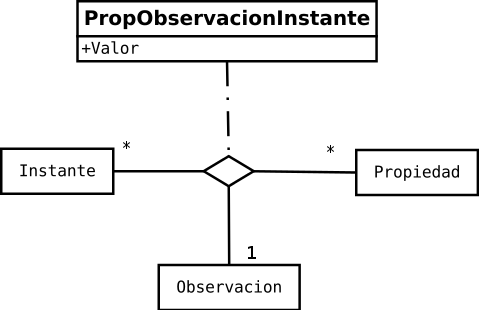
\includegraphics[width=0.7\linewidth]{./Figures/ModelodeDominio}
\caption[Modelo de dominio]{Modelo de dominio}
\label{fig:ModelodeDominio}
\end{figure}



\subsection{Librer\'{i}as usadas}
\begin{itemize}
    \item \textbf{AvalonDock:} 
    Es una librer\'{i}a que permite crear ventanas acoplables en WPF, al mas puro estilo Eclipse o Visual Studio. Es una librer\'{i}a de
    c\'{o}digo abierto y gratuita, pese a que tambi\'{e}n dispone de una versi\'{o}n profesional que es de pago. La usada en este proyecto
    ha sido la versi\'{o}n gratuita o \emph{community} como dicen ellos. La versi\'{o}n usada esta licenciada bajo licencia BSD.
    \item \textbf{Charting Toolkit}
    Es la librer\'{i}a de Microsoft para realizar distintos tipos de gr\'{a}ficas.
    \item \textbf{Infralution Localization}
    Es una libreri\'ia creada por un usuario para facilitar la localizaci\'on en WPF, ya que la manera por defecto de WPF est\'a
    muy verde.
\end{itemize}

\subsection{Patrones utilizados}

\subsubsection{MVVM}
MVVM es un patr\'{o}n de dise\~{n}o creado por Microsoft. Intenta conseguir las ventajas de Model-View-Controller como ademas una separaci\'{o}n total
de la vista del controlador. De esta forma los dise\~{n}adores de UI pueden centrar todos sus esfuerzos en crear la interfaz sin preocuparse 
del c\'{o}digo de la aplicaci\'{o}n, ya que se asume que la interfaz va a cambiar mucho durante el ciclo de vida de la aplicaci\'{o}n. Pero,
¿Si separamos totalmente la vista del modelo, como se comunican? En MVC el encargado de eso es el controlador, pero un detalle importante es 
que el c\'{o}digo referente a la vista debe tener llamadas a funciones en el lenguaje utilizado.

Y en este punto es donde la parte VM \footnote{View-Model} toma sentido. el View-Model es una abstracci\'{o}n de la vista, y que es el objetivo 
de los enlaces de datos. El View-Model expone los datos del modelo para que el creador de interfaces pueda enlazar los elementos de la UI
con los datos del modelo (bien utilizando orientaci\'{o}n a objetos o exponiendo los datos de la BD) sin escribir una sola l\'{i}nea de 
c\'{o}digo .NET.

\paragraph{Elementos de MVVM}

\begin{itemize}
    \item \textbf{Model:} Dentro del patr\'{o}n MVC corresponde al modelo de dominio utilizando orientaci\'{o}n a objetos, o a los datos
    representados por una BD.
    \item \textbf{View:} La interfaz de usuario con sus botones, cajas de texto etc.
    \item \textbf{View Model:} Es la \emph{Vista del Modelo}, siendo una abstracci\'{o}n que sirve de mediadora y que expone los datos
    del modelo a la vista, para que esta \'{u}ltima pueda utilizarlas mediante enlaces de datos simples que no requieren de c\'{o}digo, sino
    que se crean mediante XAML. Realmente, no s\'{o}lo expone los datos, si no que ademas convierte los datos del modelo, en datos de vista, listos
    para ser visualizados.
\end{itemize}

\paragraph{Cr\'{i}ticas}
Es curioso que las principales cr\'{i}ticas provengan de su creador, Josh Gossman, el cual dice que utilizar a la fuerza MVVM para operaciones simples
de UI es una exageraci\'{o}n y que si los enlaces de datos si no se gestionan correctamente puede llevar a un consumo excesivo de 
memoria de la aplicaci\'{o}n \cite{MVVM:Criticism}

\subsubsection{Iterator}
Si bien el titulo alude al patr\'{o}n \emph{Iterator} .NET no dispone como Java de la interfaz \texttt{Iterable}.
En cambio, dispone de una interfaz llamada \texttt{IEnumerator<>} que ofrece toda la funcionalidad b\'{a}sica del iterator,
y con algunas funcionalidades extra.

He decidido utilizar este patr\'{o}n por los siguientes motivos:
\begin{enumerate}
    \item \textbf{Abstracci\'{o}n:}
    Al utilizar este patr\'{o}n podemos obtener los elementos de un contenedor, que puede ser un \texttt{array}, una \texttt{LinkedList<>}... sin
    exponer su representaci\'{o}n interna, aumentando la seguridad y previniendo que una clase tenga acceso a cosas que no deba.
    
    \item \textbf{Facilidad de uso:}
    Siempre es preferible utilizar cosas que nos provea el \emph{framework}, ya que no es necesario perder el tiempo en banalidades como 
    recorrer una lista, y probablemente lo haremos menos eficientemente que lo actualmente programado. De todas formas, si necesitamos
    recorrerlo de una manera particular, y que sabemos hacerlo muy eficientemente, no hay problema en no seguir el patr\'{o}n, ya que no son
    normas, si no recomendaciones.
    
    \item \textbf{Prevenci\'{o}n de errores:}
    Relacionado con lo anterior. Si se pierde el tiempo a\~{n}adiendo l\'{i}neas extra la probabilidad de que cometamos un error 
    aumenta. Y aunque no haya sido probado emp\'{i}ricamente, se tiende a pensar que \emph{¿Como me voy a equivocar en recorrer un array? ¡Pero si est\'{a} perfecto!}. 
    Y ello llevar\'{a} a malgastar m\'{a}s aun algo tan preciado como tiempo. Pero al menos servir\'a para darse cuenta del error y 
    se ver\'a lo \'{u}tiles que son los patrones.
\end{enumerate}

\subsection{SOLID}
SOLID es un acr\'{o}nimo mnem\'{o}nico acu\~{n}ado a comienzos de la d\'{e}cada de los 2000 por Robert C. Martin \cite{SOLID:ADefinition}
que representa cinco principios b\'{a}sicos de la programaci\'{o}n orientada a objetos y el dise\~{n}o de software.

SOLID merece un apartado en esta memoria ya que se ha intentado cumplir en el mayor grado posible los cinco principios.
\cite*{Art:Programming}

Los principios son los siguientes:
\subsubsection{Single responsibility principle}
Traducido al castellano: Princpio de responsabilidad \'{u}nica. El nombre puede llevar a enga\~{n}o ya que Martin define como \emph{responsabilidad}
a una \emph{raz\'{o}n de cambio} \cite{SOLID:SRP}. Martin, concluye que una clase, debiera tener, una, y solamente una raz\'{o}n para cambiar.

Por ejemplo, imaginemos que disponemos de una clase, o m\'{o}dulo que compila e imprime un informe. Ese informe puede cambiar por dos razones,
de estilo, o de contenido. 

El principio de responsabilidad \'{u}nica dice que una clase solo debiera cambiar por un motivo, y por tanto tendr\'{i}amos que separar el m\'{o}dulo
en dos: El que compila el informe, y el que lo imprime.

Utilizando este principio volveremos nuestro c\'{o}digo mas robusto, ya que un cambio en una clase, no deber\'{i}a afectar a la salida, y por tanto
los siguientes m\'{o}dulos que se alimenten de esa clase.

\subsubsection{Open/Closed principle}
El principio abierto / cerrado \cite{SOLID:OCP} implica que una clase est\'{a} abierta a la extensi\'{o}n pero cerrada a la modificaci\'{o}n. Ya que un cambio en el
funcionamiento de una clase har\'{i}a tambalear la estabilidad de nuestro software.

\subsubsection{Liskov's substitution principle}
El principio de sustituci\'{o}n de Liskov \cite{SOLID:LSP} \footnote{\url{http://pmg.csail.mit.edu/~liskov/}} sostiene que cualquier subtipo de una clase
debe poder sustituir a su supertipo sin que haya un cambio de comportamiento.

M\'{a}s formalmente: Si \textbf{S} es un subtipo de \textbf{T} entonces \textbf{T} puede sustituirse por \textbf{S} y 
conservar su exactitud, tarea que realiza etc.

\subsubsection{Interface segregation principle}
El principio de segregaci\'{o}n de interfaces dice que es mejor tener muchas interfaces espec\'{i}ficas, que una gran interfaz que contenga todo \cite{SOLID:ISP}.

De esta manera evitamos que haya partes del software que dependan de m\'{e}todos que no influyen en esa clase.

\subsubsection{Dependency inversion principle}
El principio de Inversi\'{o}n de dependencia dice que:
\begin{enumerate}
    \item Los m\'{o}dulos de alto nivel no deben depender en m\'{o}dulos de bajo nivel. Ambos deben depender de abstracciones
    \item Las abstracciones no deben depender en los detalles. Los detalles deben depender de las abstracciones.
\end{enumerate}
\cite{SOLID:DIP}
